\begin{figure}[h!]
\centering
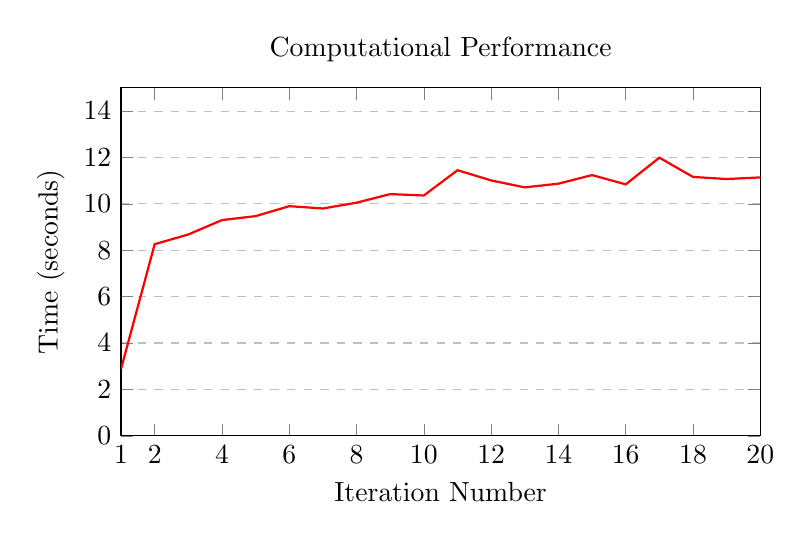
\begin{tikzpicture}
\begin{axis}[
    title={Computational Performance},
    xlabel={Iteration Number},
    ylabel={Time (seconds)},
    xmin=1, xmax=20,
    ymin=0, ymax=15,
    xtick={1,2,4,6,8,10,12,14,16,18,20},
    ytick={0,2,4,6,8,10,12,14},
    legend pos=south east,
    ymajorgrids=true,
    grid style=dashed,
    width=0.8\textwidth,
    height=6cm
]

\addplot[
    color=red,
    mark=circle,
    thick
    ]
    coordinates {
    (1,2.88)(2,8.26)(3,8.68)(4,9.30)(5,9.47)(6,9.90)(7,9.8)(8,10.05)
    (9,10.42)(10,10.36)(11,11.45)(12,11.01)(13,10.71)(14,10.87)(15,11.24)
    (16,10.84)(17,11.99)(18,11.16)(19,11.07)(20,11.14)
    };

\end{axis}
\end{tikzpicture}
\caption{Processing time for each of the 20 K-means iterations. The increase
in execution time observed indicates that from iteration 2 onwards, the CPU
temperature reaches its 100--101°C limit, triggering thermal throttling.}
\label{fig:time_per_iteration}
\end{figure}